\documentclass[12pt, titlepage]{article}

\usepackage{fullpage}
\usepackage[round]{natbib}
\usepackage{multirow}
\usepackage{booktabs}
\usepackage{tabularx}
\usepackage{graphicx}
\usepackage{float}
\usepackage{hyperref}
\usepackage[normalem]{ulem}
\hypersetup{
    colorlinks,
    citecolor=black,
    filecolor=black,
    linkcolor=red,
    urlcolor=blue
}
\usepackage[round]{natbib}

\newcounter{acnum}
\newcommand{\actheacnum}{AC\theacnum}
\newcommand{\acref}[1]{AC\ref{#1}}

\newcounter{ucnum}
\newcommand{\uctheucnum}{UC\theucnum}
\newcommand{\uref}[1]{UC\ref{#1}}

\newcounter{mnum}
\newcommand{\mthemnum}{M\themnum}
\newcommand{\mref}[1]{M\ref{#1}}

\title{SE 3XA3: Software Requirements Specification\\Title of Project}

\author{Team \# 211, Camera Crew
		\\ Faisal Jaffer, jaffem1
		\\ Dominik Buszowiecki, buszowid
		\\ Pedram Yazdinia, yazdinip
		\\ Zayed Sheet, sheetz
}

\date{\today}

%\input{../../Comments}

\begin{document}

\maketitle

\pagenumbering{roman}
\tableofcontents
\listoftables
\listoffigures

\newpage

\begin{table}[h]
\caption{\bf Revision History}
\begin{tabularx}{\textwidth}{p{3cm}p{2cm}X}
\toprule {\bf Date} & {\bf Version} & {\bf Notes}\\
\midrule
3/13/2020 & 1.0 & Initial documentation\\
4/6/2020 & 1.2 & Revision 1\\
\bottomrule
\end{tabularx}
\end{table}

\newpage


\pagenumbering{arabic}

\section{Introduction}

Decomposing a system into modules is a commonly accepted approach to developing
software.  A module is a work assignment for a programmer or programming
team~\citep{ParnasEtAl1984}.  We advocate a decomposition
based on the principle of information hiding~\citep{Parnas1972a}.  This
principle supports design for change, because the ``secrets'' that each module
hides represent likely future changes.  Design for change is valuable in SC,
where modifications are frequent, especially during initial development as the
solution space is explored.  

Our design follows the rules layed out by \citet{ParnasEtAl1984}, as follows:
\begin{itemize}
\item System details that are likely to change independently should be the
  secrets of separate modules.
\item Each data structure is used in only one module.
\item Any other program that requires information stored in a module's data
  structures must obtain it by calling access programs belonging to that module.
\end{itemize}

After completing the first stage of the design, the Software Requirements
Specification (SRS), the Module Guide (MG) is developed~\citep{ParnasEtAl1984}. The MG
specifies the modular structure of the system and is intended to allow both
designers and maintainers to easily identify the parts of the software.  The
potential readers of this document are as follows:

\begin{itemize}
\item New project members: This document can be a guide for a new project member
  to easily understand the overall structure and quickly find the
  relevant modules they are searching for.
\item Maintainers: The hierarchical structure of the module guide improves the
  maintainers' understanding when they need to make changes to the system. It is
  important for a maintainer to update the relevant sections of the document
  after changes have been made.
\item Designers: Once the module guide has been written, it can be used to
  check for consistency, feasibility and flexibility. Designers can verify the
  system in various ways, such as consistency among modules, feasibility of the
  decomposition, and flexibility of the design.
\end{itemize}

The rest of the document is organized as follows. Section
\ref{SecChange} lists the anticipated and unlikely changes of the software
requirements. Section \ref{SecMH} summarizes the module decomposition that
was constructed according to the likely changes. Section \ref{SecConnection}
specifies the connections between the software requirements and the
modules. Section \ref{SecMD} gives a detailed description of the
modules. Section \ref{SecTM} includes two traceability matrices. One checks
the completeness of the design against the requirements provided in the SRS. The
other shows the relation between anticipated changes and the modules. Section
\ref{SecUse} describes the use relation between modules.
\subsection{Software Overview}
OpenCameraRefined is designed to change the way we capture pictures through our phones. Using image processing algorithms and machine learning, the team is focused on enabling the software to process and recognize a certain gesture in real time. In addition, the software is designed to offer the user with real time filters, mainly using existing packages such as OpenCV. Some initial gestures recognized by the software can include Smile, Thumbs up or Wave. 

OpenCamera is an open-source Andorid application that provides Camera functionality outside the stock camera applications in varous phones. Android system initiates its program within an Activity starting with a call on onCreate() callback method. There is a sequence of callback methods that start up an activity and a sequence of callback methods that tear down an activity. This model is loosely based on MVC architecture with the controller being the Activity class, View being the resources and widgets and model being the entities or Classes with main Business Logic. Consequently, the modifications made follow the same principles. 
\section{Anticipated and Unlikely Changes} \label{SecChange}

This section lists possible changes to the system. According to the likeliness
of the change, the possible changes are classified into two
categories. Anticipated changes are listed in Section \ref{SecAchange}, and
unlikely changes are listed in Section \ref{SecUchange}.

\subsection{Anticipated Changes} \label{SecAchange}

Anticipated changes are the source of the information that is to be hidden
inside the modules. Ideally, changing one of the anticipated changes will only
require changing the one module that hides the associated decision. The approach
adapted here is called design for
change.


\begin{description}
\item[\refstepcounter{acnum} \actheacnum \label{acHardware}:] The specific
  hardware on which the software is running.
\item[\refstepcounter{acnum} \actheacnum \label{acGesture}:] \sout{The format of the initial input data.} \textcolor{red}{The gestures (smiling, thumbs up, wave, ...) recognized at any time by the system.}
\item[\refstepcounter{acnum} \actheacnum \label{acGestureNumber}:] The number of gestures that can be detected by the model concurrently at any given time.
\item[\refstepcounter{acnum} \actheacnum \label{acFilter}:] \sout{The gestures recognized by the algorithm.} \textcolor{red}{Addition of new filters that allow for different changes to the live preview.}
\item[\refstepcounter{acnum} \actheacnum \label{acFilterNumber}:] The number of filters available to be applied. 
\item[\refstepcounter{acnum} \actheacnum \label{acTrigger}:] \textcolor{red}{Trigger gestures used to trigger different actions such as filter change or image capture.}
\item[\refstepcounter{acnum} \actheacnum \label{acUI}:] Modifications to the UI, including extra functionality buttons that manually trigger different functions. \item[\refstepcounter{acnum} \actheacnum \label{acDraw}:] \textcolor{red}{The render protocols used to draw the real time filters. }
\item[\refstepcounter{acnum} \actheacnum \label{acSave}:] \textcolor{red}{The write protocols used to capture and save the live preview with the filter applied. }
\end{description}

\subsection{Unlikely Changes} \label{SecUchange}

\begin{description}
\item[\refstepcounter{ucnum} \uctheucnum :] Input/Output devices
  (Input: Camera, Output: Memory, Screen).
\item[\refstepcounter{ucnum} \uctheucnum :] Constant presence of a source input external to the system
\item[\refstepcounter{ucnum} \uctheucnum :] \sout{The implementation and output of gesture recognition will remain the same as this is used throughout several modules, and will require many modifications to change.} \textcolor{red}{The implementation of the trained model used to detect different gestures.}
\item[\refstepcounter{ucnum} \uctheucnum :] \sout{The user interface and settings will remain the same as the original Open Source Camera application in order to keep the application consistent and straightforward.} \textcolor{red}{The original user interface from Open Camera, excluding the added filter button.}
\item[\refstepcounter{ucnum} \uctheucnum :] \sout{Zoom and slow motion features will remain the same as this is outside the scope of this project.} \textcolor{red}{Advanced functionalities of the camera including Zoom, contrast change and etc. }
\item[\refstepcounter{ucnum} \uctheucnum :] \textcolor{red}{The actual training of the  gesture model to detect new gestures. }
\item[\refstepcounter{ucnum} \uctheucnum :] \textcolor{red}{Render protocols used to draw unfiltered preview. }
\item[\refstepcounter{ucnum} \uctheucnum :] \textcolor{red}{Read and Write protocols used to edit old pictures or save new pictures. }
\end{description}

\section{Module Hierarchy} \label{SecMH}

This section provides an overview of the module design. Modules are summarized
in a hierarchy decomposed by secrets in Table \ref{TblMH}. The modules listed
below, which are leaves in the hierarchy tree, are the modules that will
actually be implemented.

\begin{description}

\item [\refstepcounter{mnum} \mthemnum \label{mGC}:] Gesture Controller
\item [\refstepcounter{mnum} \mthemnum \label{mR}:] Recognition
\item [\refstepcounter{mnum} \mthemnum \label{mC}:] Classifier 
\item [\refstepcounter{mnum} \mthemnum \label{mCC}:] Classifier Constants
\item [\refstepcounter{mnum} \mthemnum \label{mF}:] \sout{Filter} \textcolor{red}{Image Filter Controller}
\item [\refstepcounter{mnum} \mthemnum \label{mFC}:] Filter Constants
\item [\refstepcounter{mnum} \mthemnum \label{mHH}:] Hardware Hiding Module
\end{description}


\begin{table}[h!]
\centering
\begin{tabular}{p{0.3\textwidth} p{0.6\textwidth}}
\toprule
\textbf{Level 1} & \textbf{Level 2}\\
\midrule

{Hardware-Hiding Module} & ~ \\
\midrule

\multirow{2}{0.3\textwidth}{Behaviour-Hiding Modules} & Classifier Constants\\
~ & Recognition\\
~ & Filter Constants\\
\midrule

\multirow{2}{0.3\textwidth}{Software Decision Modules} & Classifier\\
~ & Gesture Controller\\
~ & \sout{Filter} \textcolor{red}{Image Filter Controller}\\
\bottomrule






\end{tabular}
\caption{Module Hierarchy}
\label{TblMH}
\end{table}

\section{Connection Between Requirements and Design} \label{SecConnection}

The design of the system is intended to satisfy the requirements developed in
the SRS. In this stage, the system is decomposed into modules. The connection
between requirements and modules is listed in Table \ref{TblRT}.

\section{Module Decomposition} \label{SecMD}

Modules are decomposed according to the principle of ``information hiding''
proposed by \citet{ParnasEtAl1984}. The \emph{Secrets} field in a module
decomposition is a brief statement of the design decision hidden by the
module. The \emph{Services} field specifies \emph{what} the module will do
without documenting \emph{how} to do it. For each module, a suggestion for the
implementing software is given under the \emph{Implemented By} OpenCameraRefined. If the
entry is \emph{OS}, this means that the module is provided by the operating
system or by standard programming language libraries.  Also indicate if the
module will be implemented specifically for the software.

Only the leaf modules in the
hierarchy have to be implemented. If a dash (\emph{--}) is shown, this means
that the module is not a leaf and will not have to be implemented. Whether or
not this module is implemented depends on the programming language
selected.

\subsection{Hardware Hiding Modules (\mref{mHH})}

\begin{description}
\item[Secrets:]The data structure and algorithm used to implement the virtual
  hardware.
\item[Services:]Serves as a virtual hardware used by the rest of the
  system. This module provides the interface between the hardware and the
  software. So, the system can use it to display outputs or to accept inputs.
\item[Implemented By:] OS
\end{description}

\subsection{Behaviour-Hiding Module}

\begin{description}
\item[Secrets:]The contents of the required behaviours.
\item[Services:]Includes programs that provide externally visible behaviour of
  the system as specified in the software requirements specification (SRS)
  documents. This module serves as a communication layer between the
  hardware-hiding module and the software decision module. The programs in this
  module will need to change if there are changes in the SRS.
\item[Implemented By:] --
\end{description}

\subsubsection{Recognition Module(\mref{mR})}

\begin{description}
\item[Secrets:]The data and the state stored in the object.
\item[Services:]Provides access to the location, title and confidence of self.
\item[Implemented By:] OpenCameraRefined
\end{description}

\subsubsection{Filter Constants Module(\mref{mFC})}

\begin{description}
\item[Secrets:]The predefined stored filter matrices 
\item[Services:]Provides access to the predefined filters.
\item[Implemented By:] OpenCameraRefined
\end{description}

\subsubsection{Classifier Constants Module (\mref{mCC})}

\begin{description}
\item[Secrets:]The file location of the model inference and the label.
\item[Services:]Provides access to the file location strings.
\item[Implemented By:] OpenCameraRefined
\end{description}


\subsection{Software Decision Module}

\begin{description}
\item[Secrets:] The design decision based on mathematical theorems, physical
  facts, or programming considerations. The secrets of this module are
  \emph{not} described in the SRS.
\item[Services:] Includes data structure and algorithms used in the system that
  do not provide direct interaction with the user. 
  % Changes in these modules are more likely to be motivated by a desire to
  % improve performance than by externally imposed changes.
\item[Implemented By:] --
\end{description}

\subsubsection{Classifier Module(\mref{mC})}

\begin{description}
\item[Secrets:]The current sate of the running TensforFlow model.
\item[Services:]Provides methods to run classifications on images.
\item[Implemented By:] OpenCameraRefined
\end{description}

\subsubsection{\sout{Filter Module} \textcolor{red}{Image Filter Controller Module}(\mref{mF})}

\begin{description}
\item[Secrets:]The state of the current filter in view.
\item[Services:]Provides method to change the current filter.
\item[Implemented By:] OpenCameraRefined
\end{description}

\subsubsection{Gesture Controller Module (\mref{mGC})}

\begin{description}
\item[Secrets:]The flow of the information from module to module.
\item[Services:]Responsible for dispatching classification and actions based on the classification.
\item[Implemented By:] OpenCameraRefined
\end{description}


\section{Traceability Matrix} \label{SecTM}

This section shows two traceability matrices: between the modules and the
requirements and between the modules and the anticipated changes.

% the table should use mref, the requirements should be named, use something
% like fref
\begin{table}[H]
\centering
\begin{tabular}{p{0.2\textwidth} p{0.6\textwidth}}
\toprule
\textbf{Req.} & \textbf{Modules}\\
\midrule
REQ1 & \mref{mGC}, \mref{mR}, \mref{mC}, \mref{mCC}, \mref{mHH}\\
REQ2 & \mref{mGC}, \mref{mR}, \mref{mC}\\
REQ3 & \mref{mHH}\\
REQ4 & \mref{mHH}\\
REQ5 & \mref{mGC}, \mref{mR}, \mref{mC}, \mref{mCC}, \mref{mHH}\\
REQ6 & \mref{mF} \mref{mHH}\\
REQ7 & \mref{mGC}, \mref{mR}, \mref{mC},  \mref{mF}, \mref{mHH}\\
REQ8 & \mref{mGC}, \mref{mF}, \mref{mHH}\\
REQ9 & \mref{mGC}, \mref{mF}, \mref{mHH}\\
REQ10 & \mref{mF}, \mref{mFC}, \mref{mHH}\\
REQ11 & \mref{mHH}\\
REQ12 & \mref{mGC}, \mref{mF}, \mref{mHH}\\
REQ13 & \mref{mGC}, \mref{mF}, \mref{mHH}\\
\bottomrule
\end{tabular}
\caption{Trace Between Requirements and Modules}
\label{TblRT}
\end{table}

\begin{table}[H]
\centering
\begin{tabular}{p{0.2\textwidth} p{0.6\textwidth}}
\toprule
\textbf{AC} & \textbf{Modules}\\
\midrule
\acref{acHardware} & \mref{mHH}\\
\acref{acGesture} & \mref{mR} \\
\acref{acGestureNumber} & \mref{mGC}\\
\acref{acFilter} & \mref{mFC}\\
\acref{acFilterNumber} & \mref{mFC}\\
\acref{acTrigger} & \mref{mGC} \\
\acref{acUI} & \mref{mF} \\
\acref{acDraw} & \mref{mF} \\
\acref{acSave} & \mref{mHH} \\
\bottomrule
\end{tabular}
\caption{Trace Between Anticipated Changes and Modules}
\label{TblACT}
\end{table}

\section{Use Hierarchy Between Modules} \label{SecUse}

In this section, the uses hierarchy between modules is
provided. \citet{Parnas1978} said of two programs A and B that A {\em uses} B if
correct execution of B may be necessary for A to complete the task described in
its specification. That is, A {\em uses} B if there exist situations in which
the correct functioning of A depends upon the availability of a correct
implementation of B.  Figure \ref{FigUH} illustrates the use relation between
the modules. It can be seen that the graph is a directed acyclic graph
(DAG). Each level of the hierarchy offers a testable and usable subset of the
system, and modules in the higher level of the hierarchy are essentially simpler
because they use modules from the lower levels.

\begin{figure}[H]
\centering
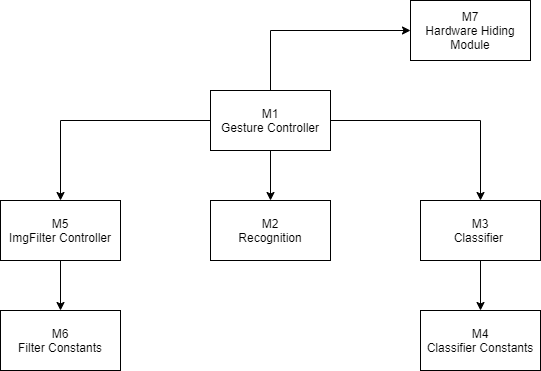
\includegraphics[width=0.7\textwidth]{UsesHierarchy.png}
\caption{Use hierarchy among modules}
\label{FigUH}
\end{figure}

%\section*{References}

\bibliographystyle {plainnat}
\bibliography {MG}

\end{document}